\section{Grundlagen}

\subsection{Genetische Algorithmen}

Genetische Algorithmen sind eine Klasse von Optimierungsalgorithmen, die sich an den Mechanismen der natürlichen Evolution orientieren\cite{Simon.2013}.
Namentlich Mutation, Crossover und Selektion.
Die Begrifflichkeiten orientieren sich entsprechen an der natürlichen Evolution.
Genetische Algorithmen arbeiten typischerweise mit Populationen aus Individuen, welche sich über Generationen entwickeln.
Jedes Individuum besitzt einen Genotypen sowie einen Phänotypen.
\missingfigure{Vllt. Bild geno phäno}
Der Genotyp eines Individuums ist typischerweise ein Vektor, das Genom des Individuums genannt, der aus einzelnen Zahlen, den Genen des Individuums, besteht. Dieser stellt die genetischen Informationen eines Individuums dar. Daneben existiert in genetischen Algorithmen eine Mapping-Funktion mit der eine Genotyp in einen Phänotyp, der nichts anderes als eine konkrete Lösung des Optimierungsproblems ist, übersetzt werden kann.

\begin{algorithm}
\caption{Genetischer Algorithmus} \label{alg:geneticAlgorihtm}
\begin{algorithmic}[1]
	\Procedure{GeneticAlgorithm}{$fitnessFunction,hyperparameters$}
	\State $population \gets initializePopulation$
	\State $populationFitness \gets fitnessFunction(population)$
	\For{$numberIterations$}
		\State $children \gets crossover(population,hyperparameters)$
		\State $children \gets mutate(children,hyperparameters)$
		\State $childFitness = fitnessFunction(children)$
		\State $population \gets selection(population,populationFitness,children,childFitness)$
		\State $populationFitness \gets updateFitness(population)$
	\EndFor
	\EndProcedure
\end{algorithmic}
\end{algorithm}

Die Mechanismen der Mutation und des Crossovers agieren auf der Ebene des Genotyps.
Mutation beschreibt die Situation, dass sich jedes Gen mit einer bestimmten Wahrscheinlichkeit ändern kann. 
Abhängig vom Typen des Gens, ist eine Änderung unterschiedlich formuliert, eine reelle Zahl mag sich anhand einer Normalverteilten Zufallsvariable ändern, eine natürliche Zahl mit $\pm1$ und ein Index mag einen zufälligen möglichen Index annehmen. 
Mutatation ist für einen genetischen Algorithmus wichtig, da sich durch diese neue Eigenschaften entwickeln können.

Crossover beschreibt die Situation, dass zwei oder mehr Elternindividuuen zu einem Kindindividuum kombiniert werden. 
Auch hier ist keine konkrete Implementierung nicht vorgeschrieben, wichtig ist nur, dass ein Kind als Kreuzung der Eltern erzeugt werden kann.
Das Ziel des Crossovers ist es, dass sich positive Eigenschaften in Populationen verteilen und mehrere unabhängig entstandenen positiven Mutationen in einem Individuum vereint werden.
Es ist allerdings anzumerken, dass Crossover einen optionalen Teil von genetischen Algorithmen darstellt, einige Algorithmen%, wie beispielsweise ($1 + \lambda$)-ES 
verzichten aus verschiedenen Gründen auf Crossover und mutieren ihre Populationen nur.
Diese beiden Methoden stellen sicher, dass neue Genotypen, und damit neue Lösungen generiert werden können, stellen aber keine Mechanismus zur Verfügung durch den dem Algorithmus eine Optimierungsrichtung gegeben wird.

Der Mechanismus, der der Optimierung eine Richtung gibt ist die Selektion.
Anders als die ersten beiden agiert diese auf Phänotypen, sprich ausgedrückten Lösungen.
Jeder genetische Algorithmus benötigt eine Funktion mit der Lösungen bewertet werden können.
Dies kann entweder in Form einer Fitnessfunktion, die die Güte eines Individuums berechnet, bei der höhere Werte besser sind, oder in der Form einer Kostenfunktion, die die Kosten eines Individuums berechnet und bei der entsprechend niedrigere Werte besser sind, geschehen.
Ob eine Fitness- oder Kostenfunktion genutzt wird hängt von der Problemformulierung ab, und ist letztendlich nur eine Frage der Algorithmus minimiert oder maximiert.
Mit diesen Funktionen kann für jedes Individuum eine Qualität berechnet werden, und Individuen können bezüglich dieser verglichen werden.
Durch Selektion werden in jeder Iteration dann schlechte Lösungen eliminiert, wodurch die Population sich zu Optima hinbewegt.
%Die Fitness, bzw. der Kosten jedes Individuums kann dann ermittelt werden und die Selektion eliminiert dann schlechte Lösungen, sprich solche mit niedriger Fitness, bzw. hohen Kosten.
Selektion ist häufig nicht so simpel, dass einfach die besten Individuen ausgewählt werden.
Die in \ref{sub:divergetnGeneticAlgorithms} besprochenen Ansätze zum Diversitätsmanagement, berücksichtigen Diversität von Populationen und können diverse Lösungen bevorzugt auswählen.

In der Gesamtschleife werden also in jeder Generation per Crossover Kinder erzeugt, die daraufhin mutiert werden.
Für diese Kinder wird dann eine Fitness berechnet.
Daraufhin werden durch die Selektion die besten Individuen ermittelt, welche zur nächste Elterngeneration werden.
Diese Schleife wird solange wiederholt bis das Maximum an Generationen erreicht ist.

\subsubsection{Divergente genetische Algorithmen}

\label{sub:divergentGeneticAlgorithms}

Eine sehr häufige Anforderung an genetische Algorithmen ist die Einbindung von Divergenz, bzw. Diversität.
Dies hat verschiedene Gründe.
Einerseits führt eine niedrige Diversität der Individuen dazu, dass nur ein kleiner Bereich des Suchraums, nämlich der in dem die Individuen liegen abgesucht wird.
Sehr homogene Populationen können dadurch einfach in lokalen Optima stagnieren, da andere Optima zu weit im Suchraum entfernt sind.
In einer diversen Population ist das Springen aus lokalen Optima hingegen einfacher, und selbst wenn Populationen stagnieren, dann geschieht dies in mehreren Optima gleichzeitig, wodurch die Wahrscheinlichkeit in einem im globalen Vergleich gutes lokalen Optimum zu finden steigt.
Auch ist es nicht unbedingt wünschenswert eine sehr homogene Population als Ergebnis zu erhalten, da die Individuen mit hoher Wahrscheinlichkeit aller der gleichen Lösungsklasse angehören.
Wenn man eine diverse Population aus Individuen erhält können Aussagen über unterschiedliche Lösungsklassen getroffen werden, Lösungsklassen und ihre Qualität können miteinander verglichen werden, und je nachdem kann größere Erkenntnis erlangt werden, was eine qualitativ hochwertige Lösung ausmacht wodurch wiederum das gestellte Problem besser verstanden werden kann.

Es existieren verschiedenste Ansätze um Diversität zu gewährleisten, welche sind grundsätzlich in genotypische und phänotypische Ansätze aufteilen lassen, abhängig davon wo Diversitätsmanagement stattfindet.
Ansätze wie Niching\cite{Shir.2012}, gewährleisten genotypische Diversität durch die Ermittlung der genetischen Ähnlichkeit zweier Individuen.
Das hat den Vorteil, dass der Genotyp eines Individuums typischerweise ein Vektor ist, und eine Vielzahl von Ähnlichkeitsmetriken für Vektoren existiert.
Dadurch fällt die Definition, was Diversität ausmacht sehr leicht.
Auch ist die Berechnung einer Distanz zwischen Vektoren sehr effizient, was vorteilhaft ist, da die Berechnung von Diversität typischerweise sehr häufig stattfinden muss.
Allerdings hat es den Nachteil, dass, besonders wenn die Genotyp-zu-Phänotyps-Mapping Funktion komplex ist, genetische Distanz nicht funktionaler Distanz zwischen Lösungen enspricht.
D. h. es besteht die Möglichkeit, dass genetisch unähnliche Individuen trotzdem in die gleiche Lösungsklasse fallen.
Deshalb wurden Ansätze wie Novelty-Search\cite{Lehman.2011} oder MAP-Elites\cite{Mouret.4202015} zum Diversitätsmanagement vorgeschlagen, die Diversität auf der Ebene, des Phänotyps bestimmen und somit funktionale Distanz messen.
Da der Phänotyp domänenspezifisch,  muss die Diversitätsmetrik für jede Domäne maßgeschneidert definiert werden, und es kann nicht auf Allgemeinlösungen zurückgegriffen werden.
Auch besteht eine erhebliche Limitierung bezüglich der Komplexität einer solche Diversitätsmetrik, da die Diversität typischerweise sehr häufig berechnet werden muss.

\subsubsection{MAP-Elites}

\label{sub:mapElites}
\begin{algorithm}
	\caption{MAP-Elites} \label{alg:mapElites}
	\begin{algorithmic}[1]
		\Procedure{MapElites}{$fitnessFunction,categorizationFunction,hyperparameters$}
		\State $map \gets $ \Comment{Initialize empty n-dimensional map}
		\State $fitness \gets $ \Comment{Initialize empty n-dimensional fitnessMap}
		\State $population \gets initializeRandomPopulation$ \Comment{Start of with randomly generated intitial samples}
		\For{$individual in population$}
			\State $f = fitnessFunction(individual)$
			\State $c = categorizationFunction(individual)$ \Comment{Categorization c is an Index to a cell in the map}
			\If{$map(c) = \emptyset \lor f < fitness(c)$} \Comment{If cell is unoccupied or this solution is better put it in cell}
				\State $map(c) \gets individual$
				\State $fitness(c) \gets f$
			\EndIf
		\EndFor
		
		\For{$numberGenerations$}
			\State $children \gets selectRandom(population,childrenPerGeneration)$ \Comment{Select samples randomly from existing solutions}
			\State $children \gets variate(children,hyperparameters)$ \Comment{Variate these children with crossover and/or mutation}
			\For{$individual in children$}
				\State $f = fitnessFunction(individual)$
				\State $c = categorizationFunction(individual)$
				\If{$map(c) = \emptyset \lor f < fitness(c)$}
					\State $map(c) \gets individual$
					\State $fitness(c) \gets f$
				\EndIf
			\EndFor
		\EndFor
		\Return $map,fitness$
		\EndProcedure
	\end{algorithmic}
\end{algorithm}
MAP-Elites (Multi-dimensional Archive of Phenotypic Elites)\cite{Mouret.4202015} ist ein genetischer Algorithmus mit phänotypischem Diversitätsmanagement.
Das bedeutet, dass die Morphologie bzw. Funktionalität einer konkreten ausgedrückten Lösung, wie beispielsweise Volumen oder Krümmung eines Bauteils, betrachtet wird.
Dazu wird der Lösungsraum entlang anhand beliebig vieler Features, deren Untersuchung als zielführend zum Verständnis des Problems befunden wird, aufgeteilt.
Diese Feature Dimensionen sind direkte Merkmale der Phänotypen von Lösungen, wie beispielsweise das Volumen eines Phänotypos in einer dreidimensionalen Domäne.
Als Features sollten solche Merkmale gewählt werden die unabhängig von der Zielfunktion sind, d. h. deren Einfluss auf die Fitness von Lösungen unklar ist.
Gerade die Untersuchung wie Merkmale mit der Fitness interagieren ist ein typisches Untersuchungsziel für MAP-Elites.
Diesen Feature-Dimensionen wird ein Minimum, Maximums sowie eine Schrittweite zugewiesen um den Lösungsraum in Zellen zu diskretisieren.
Diese Diskretisierung zu Zellen wird typischerweise Karte oder Archiv genannt.
Wichtig für MAP-Elites ist das jede Zelle nur maximal eine Lösung enthalten kann.
%Jede dieser Zellen stellt dabei eine Kombination der Eigenschaften dar.
Zu Beginn des Algorithmus werden alle Zellen leer initialisiert, im Laufe des Algorithmus werden diese nach und nach gefüllt.
Zuerst werden zufällige Individuen generiert um die Karte mit einer Initialpopulation zu befüllen.
Daraufhin werden in jeder Generation aus den momentan in der Karte enthaltenen Lösung zufällig Individuen ausgewählt um die Kindpopulation zu erzeugen.
Aus dieses ausgewählten Individuen wird eine Kindpopulation per Mutation und/oder Crossover erzeugt.
Jedes dieser Kinder wird bezüglich dessen Fitness evaluiert und dessen zugehöriger Phänotyp wird nach den gewählten Features kategorisiert.
Diese Kategoriesierung weist jedem Kind eine Zelle zu die es befüllen könnte.
Ist diese Zelle noch leer befüllt das Kind diese, befindet sich bereits ein Individuum in der Zelle, findet zwischen diesem und dem Kind lokal Konkurrenz statt.
Die lokale Konkurrenz innerhalb der Zellen ist was MAP-Elites zu einem divergenten Algorithmus macht.
Da Lösungen nur durch Lösungen verdrängt werden können, denen die gleiche Zelle zugewiesen ist, können Lösungen nur durch ihnen phänotypisch ähnliche Lösungen verdrängt werden.
Dadurch wird die phänotypische Diversität des Algorithmus gewährleistet.
Außerdem kann die Größe des Archivs während des Algorithmus nur zunehmen, da Individuen nur verdrängt werden können wenn sie durch ein anderes ersetzt werden, aber im Laufe des Algoithmus immer mehr leere Zellen befüllt werden können.
Dass bedeutet, dass die Anzahl an lokalen Optima, die der Algorithmus ermittelt hat über dessen Laufzeit wächst.

%Dadurch ist der Algorithmus divergent, denn dadurch, dass nur lokale Konkurrenz stattfindet kann ein Individuum nur durch ein phänotypisch ähnliches verdrängt werden, wodurch die phänotypische Diversität nicht sinkt.
Nicht nur wird eine Vielzahl von Lösungen generiert, die unterschiedliche Lösungsklassen abdecken, sondern die regelmäßig aufgeteilte Karte kann auch dabei helfen die Effekte, die die Features auf die Lösungsqualität haben zu verstehen.


\subsection{Surrogat-Modellierung}

\label{sub:surrogate}
Für die Selektion von Individuen innerhalb eines genetischen Algorithmus wird die Lösungsqualität dieser Individuen, typischerweise Fitness genannt, benötigt.
Außerdem findet die Auswertung der Fitnessfunktion innerhalb des genetischen Algorithmus sehr häufig statt.
Dies stellt bei relativ einfachen Fitnessfunktionen keine große Einschränkung dar, auf Problemdomänen in denen die Auswertung der Fitness eines Individuums allerdings komplexer und dadurch zeitaufwändiger wird, kann dies die Anwendbarkeit einfacher genetischer Algorithmen einschränken.

Aerodynamische Probleme, für die zeitaufwändige Simulationen nötig sind, gehören ohne Zweifel zu der Klasse von Problemen, für die die Anzahl der benötigten Funktionsauswertungen zu groß sind, als das der Algorithmus in vertretbarer Laufzeit abschließen kann.
Um genetische Taktiken auf eine solche Problemdomäne anzuwenden, wird eine Möglichkeit benötigt die benötigten Funktionsauswertungen erheblich zu reduzieren.
Eine solche Möglichkeit ist ein Surrogatmodell \cite{Jin.2011}\cite{Preen.2016}, eine Machine-Learning Modell, welches aufgrund echter Simulationsauswertungen trainiert wird, um deren Ergebnis annähernd vorherzusagen.
Eine Auswertung des Modells erfordert dabei nur einen winzigen Bruchteil des Aufwands, der für eine Simulation nötig wäre.

Die Einführung eines Surrogatmodells bringt allerdings einige Probleme mit sich.
Das wichtigste zu lösende Problem ist, wie bestimmt wird anhand welcher realen Funktionsauswertungen das Surrogatmodell trainiert wird.
Dabei müssen einige Ziele beachtet werden.
Ersten sollte das Surrogatmodell möglichst präzise sein, da es seinen Zweck für reale Funktionsauswertungen einzustehen nur erfüllen kann, wenn die Vorhersagen des Surrogatmodells ausreichend gut reale Funktionauswertungen abbilden.
Da das Surrogatmodell aber genau für den Zweck genutzt wird die Anzahl an benötigten teuren Funktionsauswertungen zu reduzieren, wäre es sinnvoll, wenn Funktionauswertungen so gewählt werde, dass sie maximalen Nutzen bringen.

\subsubsection{Exploration Exploitation Problem}

Ein häufig auftretendes Dilemma beim Lernen von unbekannten Problemen ist die Spannung zwischen Exploration und Exploitation.
Exploration beschreibt dabei die Untersuchung von unbekannten, bisher unerforschten Gebieten, um das zugrundeliegende Problem besser zu verstehen und damit Strategien besser optimieren zu können.
Exploitation beschreibt die Ausnutzung von bekannten guten Strategien, um Nutzen zu maximieren.
Die beiden Herangehensweisen stellen gegensätzliche Konzepte dar.
Je mehr Exploration durchgeführt wird, desto weniger Exploitation kann durchgeführt werden und vice-versa.
Ein zu starker Fokus auf Exploration führt allerdings dazu, dass viele niedrigwertige Gebiete erforsch werden, diese aber keinen Nutzen einbringen.
Zu viel Exploitation hingegen kann zur Folge haben lokale Gewinne über globale Gewinne zu bevorzugen.

Ein solches Problem stellt sich auch bei der Surrogatmodellierung.
So ist einerseit die Exploration unerkundeter Gebiete wichtig zur Maximierung der globalen Präzision des Modells, die Exploitation allerdings wichtig zur Untersuchung von Regionen mit hoher Fitness, da in diesen Regionen der Hauptteil der Optimierung stattfindet.
Auch ist die Anzahl an erlaubten realen Auswertungen stark begrenzt, die Reduzierung ist der Grund für die Nutzung eines Surrogatmodells.
D. h. dass die Auswertungen die durchgeführt werden maximalen Nutzen für das Surrogatmodell haben sollten.

Eine Möglichkeit mit dem Dilemma zwischen Exploration und Exploitation umzugehen ist das in \todo{cite Using Confidence Bounds forExploitation-Exploration Trade-offs} beschriebene Upper-Confidence-Bound. Dabei werden Exploration-Exploitation Probleme als statistischen Prozesse bestehend aus Mittelwert und Varianz aufgefasst.
Der Mittelwert an einem Punkt spiegelt dabei den erwarteten Nutzen wieder, eine dem Mittelwert folgende Auswahl bevorzugt also Exploitation von Bereichen in denen der erwartete Nutzen hoch ist.
Die Varianz spiegelt die Unsicherheit an einem Punkt wieder, eine Auswahl nach Varianz bevorzugt die Exploration von Bereichen in denen eine hohe Varianz auftritt, oder anders gesagt von bisher unerforschten Bereichen.
Upper-Confidence-Bound kombiniert Mittelwert und Varianz zur Bestimmung der besten Punkte, und erreicht damit eine Balance in der sowohl Exploration als auch Exploitation stattfindet.

%Durch die Auswertung von Punkten mit hoher Varianz kann die Anzahl an benötigten realen Funktionsauswertungen gering gehalten werden.
%Die Auswertung von Punkten mit hoher Varianz, sprich die Auswertung von bisher nicht erkundeten Gebieten wird Exploration genannt.
%Wenn allderdings nur die Exploration des Suchraums durchgeführt wird, wird dies dazu führen, dass viele nicht-optimale Bereiche erkundet werden.
%Da der Gaußprozess im Kontext einer Optimierung genutzt wird hat die Präzision des Gaußprozesses in Bereichen um Optima besondere Bedeutung.
%Die Verbesserung der Präzision des Gaußprozesses in optimalen Regionen wird Exploitation genannt.
%Insgesamt muss eine Abwägung zwischen der Exploration unbekannter Bereiche der Funktion und der Exploitation bekannter optimaler Bereiche der Funktion stattfinden. 
%Eine Möglichkeit einer solchen Abwägung ist Upper-Confidence-Bound \todo{cite}, einer Kombination aus Mittelwert, der Exploitation bevorzugt, und Varianz, die Exploration bevorzugt.

\subsubsection{Gaußprozesse}

\missingfigure{Visualisierung Gaußprozess}

Gaußprozesse sind ein in \cite{Rasmussen.2008} entwickeltes Machine-Learning Verfahren, mit welchem beliebige mathematische Funktionenen approximiert werden können. 
Ein großer Vorteil von Gaußprozessen ist, dass sie durch ihre Herkunft aus der Statistik die zu approximierende Funktion als Kombination aus Normalverteilungen modellieren.
Dadurch können Gaußprozesse neben einer Vorhersage, genauer gesagt dem Mittelwert der Vorhersage an einem Punkt, auch die Varianz der Vorhersage an jedem Punkt liefern.
Durch diese Eigenschaft bieten sie gute Vorraussetzungen zur Anwendung von Upper-Confidence-Bound, und können dadurch Vorhersagen welche Funktionsauswertungen den statistisch höchsten Nutzen unter Abwägung zwischen Exploration und Exploitation haben.
Damit können die benötigten Funktionsauswertungen weiter reduziert werden, beziehungsweise die Präzision des Modells bei begrenzter Zahl von Funktionsauswertungen maximiert werden.
Diese Eigenschaft stellt den Hauptvorteil von Gaußprozessen gegenüber anderen Machine-Learning Verfahren dar und ist der Grund warum Gaußprozesse als Surrogatmodell in SAIL genutzt werden.

%Dies ist für die Nutzung als Surrogatmodell genau deshalb wünschenswert, da es ein Maß der Präzision für jeden Punkt der Funktion darstellt.
%Da die Auswertung eines Punktes und die Einführung dieses in den Gaußprozess, immer den Kollaps der Varianz an diesem Punkt zu null zu Folge hat, bietet der Gaußprozess eine Möglichkeit den Präzisionsgewinn durch die Auswertung eines Punktes zu quantifizieren.


Der Hauptnachteil von Gaußprozessen ist die relativ hohe Speicher- und Rechenkomplexität \todo{komplexität}, da die Anzahl an Simulationen die durchgeführt werden können aber ohnehin durch den Rechenaufwand, der mit diesen verbunden, ist, stark limitiert ist, wird die Anzahl an Trainingsdaten so gering bleiben, dass Komplexitätsüberlegungen hinfällig sind.



\subsubsection{SAIL}

\begin{algorithm}
	\caption{MAP-Elites} \label{alg:mapElites}
	\begin{algorithmic}[1]
		\Procedure{MapElites}{$evaluate,categorizationFunction,hyperparameters$}
			\While{$numberEvaluatedSamples < totalSamples$}
				\If{$notInitialized$}
\State $evaluatedSamples \gets evaluate(randomSampling())$ \Comment Evaluate is the real costly Fitness-Function.
\Else
\State $surrogate \gets trainSurrogate(evaluatedSamples)$
\State $acquisitionMap \gets MapElites(acquisitionFunction,categorizationFunction,hyperparameters)$
\State $nextSamples \gets sampleRandomFromMap(acquisitionMap)$ \Comment SAIL utilizes Sobol-sequences to achieve optimal spread of the Sampling
\State $evaluatedSamples \gets evaluatedSamples \cup evaluate(nextSamples)$
\EndIf
			\EndWhile
		\EndProcedure
	\end{algorithmic}
\end{algorithm}

\missingfigure{Vllt. Graphik zu SAIL}

\todo{cite sail}
SAIL (Surrogate-Assisted Illumination) vereint die in \ref{sub:mapElites} und \ref{sub:surrogate} beschriebenen Ansätze, mit dem Ziel MAP-Elites in rechenintensiven Domänen anwendbar zu machen.

Zur Initialisierung SAILs werden zuerst zufällig Samples ausgewählt und evaluiert.
Um eine gleichmäßige Verteilung der Samples über den Problemraum zu garantieren werden diese Samples nicht aus einer Gleichverteilung, sondern aus einer Sobol Sequenz ausgewählt.\todo{cite sobol sequenz}
Der eigentliche Kern von SAIL ist die graduelle Verfeinerung des Surrogatmodells.
In jeder Iteration der Verfeierungsschleife wird ein Gaußprozess auf Basis aller bisher ausgewerteten Samples trainiert.
Mit diesem Gaußprozess wird MAP-Elites durchgeführt, wobei als Fitnessfunktion für die Durchführung von MAP-Elites die Akquisefunktion genutzt wird.
Dadurch wird die sogenannte Akquisekarte erzeugt, welche diverse Lösungen enthält, die die Akquisefunktion maximieren.
Aus dieser Akquisekarte werden dann mehrere Lösungen für reale Fitnessevaluationen ausgewählt.
Durch die Nutzung von Upper-Confidence-Bound als Akquisefunktion stellen diese Lösungen Optima bezüglich Exploration und Exploitation dar.
Die ausgewählten Samples werden daraufhin ausgewertet  und den bereits ausgewerteten hinzugefügt um den Gaußprozess in der nächten Iteration besser zu trainieren.
Dies kann abhängig von den verfügbaren Rechenkapazitäten beliebig oft wiederholt werden.
Am Ende poduziert diese Schleife eine Menge an echten Ausgewerteten Samples auf deren Basis der Gaußprozess trainiert werden kann.

Um am Ende Ergebnisse zu erzeugen kann MAP-Elites mit dem finalen Gaußprozess und dessen Mittelwert als Fitnessfunktion ausgeführt werden.
Der Mittelwert des Gaußprozesses an einem Punkt entspricht gerade der mittleren Vorhersage zur Fitness einer realen Auswertung an diesem Punkt.
Damit wird dann eine diverse Vorhersagekarte erzeugt, die die Optima des Gaußprozesses zeigt.
Bei korrekter Parametrisierung von SAIL, dem Gaußprozess, und einer ausreichen großen Anzahl an realen Auswertungen korrespondieren OPtima im Gaußprozess mit Optima in der realen Fitnessfunktion.

In \cite{Gaier.6152018} wurde gezeigt, dass dieser Ansatz erfolgreich auf 2D und 3D aerodynamische Domänen angewandt werden kann.
Es wurden Freiform-Deformationen auf 3D-Bauteile angewandt, welche dann wiederum bezüglich ihrer aerodynamischen Eigenschaften ausgewertet wurden, um ein Surrogat-Modell zu trainieren.


\subsection{Constraints in Optimierungsprozessen}
Constraints sind eine Möglichkeit sekundäre Optimierungsparemter, welche neben dem primären Optimierungsziel ebenfalls eingehalten werden sollen, in einen Optimierungsprozess einzuarbeiten, ohne auf multivariate Optimierung zurückgreifen zu müssen.
Constraints lassen sich grundsätzlich in Soft Constraints, bei denen die Nichteinhaltung des Constraints zur Addition von Strafwerten auf die Optimierungsfunktion führt, und Hard Constraints, die eine binäre erfüllt/nicht erfüllt Auswahl treffen.
Welche dieser beiden Arten von Constraints genutzt wird, hängt stark von der Problemstellung ab.

Auch stellt die Formulierung von Constraints häufig eine Herausforderung dar.
So müssen diese offensichtlich berechenbar sein, Constraints sind allerdings häufig nicht in mathematischer Form formuliert sondern eher in einer Art die an Requirements erinnert.
Es muss folglich zuerst eine mathematische Formulierung für den Constraint entwickelt werden, die den Constraint sow eit wie möglich entspricht.
Zweitens werden Constraints in einem typischen evolutionären Optimierungsalgorithmus sehr häufig evaluiert werden. Das bedeutet, dass die Berechnung des Constraints entweder nicht besonders rechenintensiv sein darf, oder Hilfsmechanismen integriert werden wie beispielsweise die Modellierung des Constraint durch ein Surrogatnetzwerk, wie es in SAIL für die Fitness bereits genutzt wird.

\subsubsection{Hard Constraints}

Hard Constraints führen eine binäre Auswahl durch, bei der solche Lösungen, die den Constraint nicht erfüllen disqualifziert werden.
Sie stellen eine sehr einfache Lösung zur Implementierung von Constraints dar.
An der Stelle im Algorithmus an der neue Lösungen generiert werden werden alle ungültigen Lösungen herausgefiltert.
Dies hat den Vorteil, dass ungültige Lösungen niemals in den Algorithmus einfließen, und damit weder Rechenkapazitäten für nicht-nutzbare Lösungen genutzt werden, und solche Eigenschaften, durch die eine Lösung die Constraints verletzt vom Algorithmus überhaupt nicht in Erwägung gezogen werden.


\subsubsection{Soft Constraints}
Soft Constraints disqualifizieren Lösungen, die die Constraints verletzen, nicht.
Stattdessen wird beim Nichterfüllen von Constraints ein Strafwert auf die Kostenfunktion addiert, bzw. von einer Fitnessfunktion subtrahiert.
Das Lösungen, die die Constraints nicht erfüllen, nicht disqualifiziert werden, hat den Vorteil, dass viele Optimierungmethoden iterativ zu (lokalen) Optima konvergieren\footnote{Auch ein divergentes Optimierungsverfahren wie MAP-Elites konvergiert zu Optima, es wird nur sichergestellt, das zu einer Vielzahl lokaler Optima konvergiert wird}, 
und diese auch Lösungen, die die Constraints nicht erfüllen, als Trittbretter zu Lösungen, die die Constraints erfüllen, nutzen können.

Soft Constraint eignen sich in Fällen, in denen zu Beginn keine Lösungen bekannt sind, die die Constraints erfüllen, und in denen explorativ nach Lösungen gesucht werden soll, die die Constraints erfüllen.
Auch eignen sie sich für solche Probleme, in denen qualitative Unterschiede bezüglich der Stärke der Verletzung der Constraints zwischen unterschiedlichen Lösungen exisistieren können.
So kann argumentiert werden, dass im Falle, dass ein Constraint die Einhaltung eines Schwellenwerts ist, eine Lösung, die diesen um 1 überschreitet, qualitativ besser ist als eine, die diesen um 10 überschreitet.

Eine der größten Gefahren bei Soft Constraints ist, dass diese typischerweise als Kostenfunktionen formuliert werden, deren Wert mit der eigentlichen Zielfunktion der Optimierung kombiniert wird.
Eine solche Kombination enthält immer eine Gewichtung für alle Teilfunktionen die sie ausmacht.
Ist diese Gewichtung fehlerhaft parametrisiert, kann dies dazu führen, dass Teilfunktionen über- oder unterpriorisiert werden, und Constraints vom Algorithmus ignoriert werden, oder, dass nicht mehr nach dem primären Optimierungsziel optimiert wird.


\newpage

\section{Methode}

\subsection{Domänenübergreifend}

In beiden Domänen geht es um die Deformation von dreidimensionalen Bauteilen, und die Bewertung der aerodynamischen Effekte solcher Deformationen.
D. h. es wird eine robuste Methode benötigt um dreidimensionale Bauteile zu deformieren und solche Deformationen auf wenige Parameter reduzieren zu können.
Eine Methode, die diese Rahmenbedingungen erfüllt ist die Freiformdeformation \cite{Sederberg.1986} auf die in \ref{sub:ffd} genauer eingegangen wird, die Deformationen von komplexen geometrischen Objekten anhand Verschiebungen von Rahmenpunkten ausdrücken kann.
Für aerodynamische Simulationen wird in beiden Domänen OpenFoam verwendet, ein Open-Source Programm welches unter anderem fähig ist Windkanalsimulationen durchzuführen.
Auf die genaueren Eigenschaften von OpenFoam und den Aufbau einer passenden Simulationsumgebung wird in \ref{sub:openfoam} eingegangen.

\subsubsection{Freiformdeformation}
\label{sub:ffd}
Freiformdeformation\cite{Sederberg.1986} ist ein Verfahren zu Deformation von geometrischen Objekten.
Mithilfe der Freiformdeformation können beliebige dreidimensionale Meshes robust deformiert werden.
Dazu wird eine Box aus Kontrollpunkten erzeugt.
Jeder dieser Kontrollpunkte kann dann anhand von Verformungsparametern verschoben werden, wodurch für alle Punkte innerhalb der FFD-Box eine Verschiebung berechnet wird, die von der relativen Position des Punktes zum Kontrollpunkt abhängt.
Dadurch kann eine Deformation auf eine überschaubare Anzahl an Deformationsparametern reduziert werden.
Außerdem kann eine Deformation auf einige bestimmte Punkte und/oder Richtungen
\footnote{Deformation in x, y, z finden jeweils separat statt}
beschränkt werden, um die Komplexität weiter zu reduzieren.
Dadurch das nur die Punkte des Meshes ihre Position ändern, hat das Verfahren, den Vorteil das die Dreiecke erhalten bleiben und somit beispielsweise das Entstehen von Löchern bei korrekter Anwendung praktisch ausgeschlossen ist.

\subsubsection{OpenFOAM}
\label{sub:openfoam}
OpenFoam \cite{OpenCFD.} ist eine Open-Source Programm zur Durchführung von Fluiddynamiksimulationen.
Berechnungen in OpenFOAM sind in sogenannten "Cases" organisiert auf die nacheinander OpenFoam-Funktionen angewandt werden
Diese Cases bestehen aus einer Basisstruktur, die Initiale Startparameter, sowie Dateien zur Steuerung von OpenFoam enthalten.
%Diese basis ist in den Ordnern \textit{domains/wheelcase/pe} und \textit{domains/escooter/pe} zu finden.
Diese Basis enthält typischerweise Skripts um die gesamte Kette aus verschiedenen OpenFoam Funktionen, die zur Durchführung einer Simulation notwendig sind, auszuführen (Allrun), sowie ein Skript, welches den Case wieder in den Case wieder in den Startzustand versetzt (Allclean).
Außerdem enthält diese basis den Ordner system, der C++-Dictionaries enthält, mit denen die einzelnen OpenFoam Funktionen parametrisiert und gesteuert werden.
Zuletzt befindet sich in diesem Ordner auch noch der Initiale Startzustand mit dem die Simulation beginnt (0org)
OpenFOAM bietet native Unterstützung von Parallelität über die MPI-Bibliothek \cite{OpenMPI.}.
Neben den Funktionen um die korrekte Aufteilung eines Cases auf mehrere Prozessoren aufzuteile und am Ende wieder zu rekonstruieren sind zwei Funktionen und deren dazugehörige Dateien hervorzuheben.

Die zwei wichtigsten genutzten OpenFoam-Funktionen sind \path{snappyHexMesh} und \path{simpleFoam}.
Mit snappyHexMesh, dessen Parametrisierung in \path{snappyHexMeshDict} zu finden ist, wird aus dem STL das für die Fluiddynamiksimulation benötigte Mesh generiert. Über snappyHexMesh kann die Auflösung des in der Fluiddynamiksimulation genutzen Meshes kontrolliert werden.
Die Paramtrisierung von snappyHexMesh ist deshalb besonders wichtig, da die Auflösung des Meshes


Die zweite dieser Funktionen ist die eigentliche Fluiddynamiksimulation welche durch die Datei \path{fvSolution} gesteuert wird. 
Es stehen verschiedene Simulationen für verschiedene Zwecke zur Verfügung.
Für den hier benötigten Zweck ist simpleFoam vollkommen ausreichend.

\subsubsection{Parametrisierung des Gaußprozesses}


\subsection{Radkästen des Velomobils}

\begin{figure}[h]
	\centering
	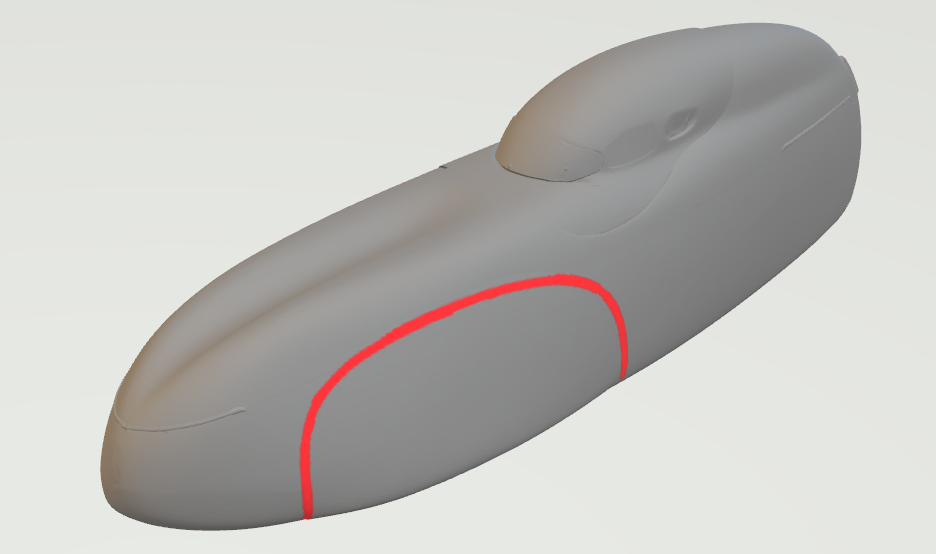
\includegraphics[width=.8\linewidth]{bilder/velo_wheelcase}
	\caption{Radkasten des Velomobils}
	\label{fig:wheelcase}
\end{figure}

Die erste Problemdomäne stellt die Optimierung der Radkästen eines Velomobils dar.
Da die momentanen Radkästen den Lenkausschlag des Velomobils erheblich einschränken, besteht das Ziel hierbei Radkästen zu generieren, die den maximalen, oder zumindest einen weiteren Lenkausschlag als den momentan möglichen, ermöglichen und dabei trotzdem gute aerodynamische Eigenschaften aufweisen.
Es ist zu erwarten, dass eine zusätzliche Fokussierung auf ein zweites Ziel, mit einer Qualitätsabnahme des ersten Ziels verbunden ist.
Trotzdem ergibt die Einführung eines Constraints nur Sinn, wenn die Abnahme an Optimalität bezüglich des Primärziels gering genug ist um eine Zunahme an Optimalität bezüglich des Sekundärziels vertretbar zu machen.
Das Ziel besteht also darin Lösungen zu entwickelt, welche durch minimalen Fitnessverlust einen maximalen Constraintgewinn möglich machen.

\subsubsection{Struktur}

%\begin{figure}[h]
%%	\centering
%	\dirtree{%
%		.1 placeholder.
%	}
%\caption{Struktur von domains/wheelcase}
%\label{fig:dir_wheelcase}
%\end{figure}

%Alle spezifischen Daten zur wheelcase Domäne sind in \path{domains/wheelcase} zu finden.
%Auf der höchsten Ebene des Verzeichnisses sind die generellen Skripte für SAIL zu finden.
%Im Unterverzeichnis \path{ffd} befinden sich die STLs, die für die Freiformdeformation und Berechnung des Constraints benötigt werden.
%Alle Dateien zur Berechnung des Constraints leigen in \path{constraint}
%Der Basiscase für OpenFoam ist zu finden \path{pe/v1906}.
%Im Ordner \path{configs} befinden sich verschiedene Konfigurationen für die Freiformdeformation
%Eine solche Konfiguration enthält die Parametrisierung für die Freiformdeformation, sowie die Funktion zur Erzeugung einer konkreten Deformation aus einem Genom.
%Das letzte Unterverzeichnis ist \path{experiment}, was das Skript zum Starten eines Laufs, sowie Job-Skripte zur Ausführung als Slurm-Jobs

\subsubsection{OpenFOAM}

\subsubsection{Constraint}
\missingfigure{Radausschlagvolumen mit und ohne velomobil}
Zur Erfüllung des Constraints wurden alle möglichen Radausschläge als Volumen modelliert.
Dafür wurden aus einer Kugel entsprechend der maximalen Radausschlags nach rechts und links ein dreieckiges Stück ausgeschnitten.
Zusätzlich wurde die innere Hälfte der Kugel entfernt, da dort keine Überschneidungen stattfinden, und durch deren Entfernen, Berechnungen mit dieses Volumen effizienter sind.
Dieses Volumen ist in Abb. \ref{fig:steering_volume} alleine, in Abb. \ref{fig:steering_volume_with_velo} zusammen mit dem restlichen Velomobil zu sehen.
Es ist klar zu Erkennen, dass dieses Volumen die unverformten Radkästen schneidet, da diese den maximalen Lenkausschlag nicht ermöglichen.
 

\begin{table}[h]
	\begin{tabularx}{.5\textwidth}{ll}\hline
		
		Position\footnote{Urpsprung des Koordinatensystems auf Boden an der Spitze des Velomobils. Linkshändiges Koordinatensystem mit z Höhenachse und Velomobil in -x-Richtung ausgerichtet} & \\
		\hline
		x &	$926mm$ \\
		y &	$343mm$ \\
		z &	$205mm$	\\
	\end{tabularx}
	\begin{tabularx}{.5\textwidth}{ll}\hline
		Rotation & \\ \hline
		$\phi$ & $16,6\degree$ \\
		$\theta$ & $0\degree$ \\
		$\psi$ & $0\degree$ \\
	\end{tabularx}
	\begin{tabularx}{.5\linewidth}{ll}
		Radius des Rads & $230mm$ \\
		Radausschlag & $\pm24,37\degree$\\
		
	\end{tabularx}

\label{tab:wheel_params}
\caption{Parameter Radausschlag}
\end{table}

Da ein Ziel darin bestand, den Constraint nicht als binäres, erfüllt/nicht erfüllt Problem zu definieren, da zwischen zwei Lösungen, die den Constraint nicht erfüllen trotzdem qualitative Unterschiede bestehen können wie stark der Constraint verletzt wird, wird als Constraint das Differenzvolumen des Radausschlags minus verformten Radkastens gewählt.
Da alle generierten Verformungen der Radkästen symmetrisch sind, wird der Constraint jeweils nur für den rechten Radkasten berechnet.
Zwar besteht keine direkte Kausalität zwischen diesem Volumen und dem maximalen möglichen Radausschlag aber die Vermutung, dass eine geringeres Volumen dieser Different mit größerem möglichen Radausschlag korreliert ist liegt nahe.
Zur Berechnung der Differenz zwischen Radausschlagsvolumen und Radkasten wird die Bibliothek \textit{gptoolbox} \cite{gptoolbox.b} genutzt, zur Generierung von Tetraedermeshes zur Volumenberechnung \textit{TetGen} \cite{Si.2015}.
Ein Beispiel des Differenzvolumens zur Constraintberechnung ist in Abb. \ref{fig:diff_volume} zu sehen.
Dieses Volumen stellt die Differenz des Radausschlagvolumens und des unverformten Radkastens dar.
Um eine Differenz berechnen zu können wurde der rechte Radkasten zu einem geschlossenen Volumen gemacht, da die Constraintberechnung in jeder Generation für jedes Kind erfolgen muss wurde der Radkasten außerdem vereinfacht um die Berechnung  des Constraints ausreichend schnell durchführen zu können.
Aus dem Volumen wird dann der Strafwert berechnet der in Relation zum Differenzvolumen des unverformten Radkastens
\footnote{Für den unverformten Radkasten beträgt das Differenzvolumen ca. $1,6L$} gesetzt wird.

Da sich der Constraint durch die Vereinfachung des Radkastens ausreichend schnell berechnen ließ, dass eine direkte Berechnung dessen für jedes Individuum zeitlich möglich war, wurde dies getan.
Das Trainieren eines zweiten Surrogatmodells zur Modellierung des Constraints hätte einen nicht unerheblichen Komplexitätszuwachs bedeutet , der an dieser Stelle nicht nötig war.
Also wurde dieser Strafwert direkt in die Fitnessfunktion integriert und als $\frac{V_{verformt}}{V_{unverformt}} * w_{constraint}$ auf die Fitness jedes Individuums addiert
\footnote{Die vorliegende SAIL-Implementation minimiert}.
Allerdings wurde der Strafwert zusätzlich noch in die Akquisefunktion, mit der einnerhalb von SAIL die Akquisekarte zur Auswahl neuer Individuen zur Auswertung stattfindet auf die gleiche Weise integriert. Das hat den Grund, dass das Gaußprozessmodell in solchen Bereichen bevorzugt Exploitation durchführen soll, die sowohl bezüglich der Aerodynamik, als auch bezüglich des Constraints eine gewisse Optimalität aufweisen, da genau in diesen Bereichen, in der finalen Auswertung von MAP-Elites solche Lösungen zu erwarten sind die bezüglich der Kombination dieser beiden Kriterien optimal sind.


\subsubsection{Wahl der Features}
%Die Kategorisierung wird von der \path{wheelcase_Categorize.m} verwaltet.

Als erste Kategorie wurde die Breite des Velomobils gewählt.
Diese Kategorie wurde deshalb gewählt, da hier sehr klare Hypothesen aufgestellt werden können, wie die Breite des Velomobils mit der Aerodynamik und dem Constraint interagiert.
Die erste Hypothese, die aufgestellt werden kann ist, dass breiteren Velomobilen die Erfüllung des Constraints leichter fällt. Es wäre also zu erwarten, dass breitere Velomobile den Constraint tendenziell besser erfüllen, als schmalere.
Auch kann die Hypothese aufgestellt werden, dass die Breite negativ mit dem Luftwiderstandsbeiwert korreliert ist.
Insgesamt wäre also zu vermuten, dass entlang dieser Achse der Luftwiderstandsbeiwert zunimmt während der Strafwert des Constraints abnimmt.
Der Test ob diese Erwartungen erfüllt sind stellt eine einfache Möglichkeit zur semantischen Verfifizierung der Ergebnisse dar.

Als zweite Kategorie wurde die x-Koordinate des breitesten Punkts gewählt.
Da das Velombil in negative x-Richtung ausgerichtet ist, bedeuten kleinere Werte hier, dass der Punkt weiter vorne liegt, größere, dass er weiter hinten liegt.
Zu dieser Kategorie lassen sich keine so direkten Hypothesen aufstellen wie zur ersteren.
Die Frage ob sich hier klare Tendenzen bezüglich den aerodynamischen Eigenschaften und/oder des Constraints aufzeigen ist auch ein Ziel der Untersuchung.

Da auch die Kategorisierung so häufig stattfindet, wird auch diese mit dem für die Berechnung des Constraints vereinfachten Modell des Radkastens durchgeführt. 
Dies stellt keinen signifikanten Verlust an Genauigkeit in der Kategorisierung dar, da sich die am feinsten gemeshten Teile des Radkastens an dessen Rändern befinden.
Gerade die sind aber die Teile des Radkastens, die am unwahrscheinlichsten den breitesten Punkt darstellen.
Auch führen minimale Genauigkeitsfehler in der kategorisierung nicht dazu, dass die von MAP-Elites geforderte Lokalität verletzt wird.
Der Geschwindigkeitsgewinn bei der Berechnung hingegen mach es möglich solche Kategorien, für die eine Verformung des Radkastens notwendig ist, zu wählen, was in Relation einen wesentlich größeren Gewinn darstellt.

\subsection{E-Roller}

\missingfigure{E-Rollerbauteil}

Die zweite Problemdomäne ist die explorative Untersuchung eines Bauteils an der Unterseite eines E-Rollers.
Hier besteht die Frage ob nicht-triviale Bauteile aerodynamische Vorteile bieten, und welche Eigenschaften solche Bauteile aufweisen.

\subsubsection{Setup}
\subsubsection{OpenFOAM}
\subsubsection{Constraint}
\subsubsection{Wahl der Features}





